\chapter{Herausforderungen und Lösungen im Bereich Deep Learning}

\section{Overfitting und Underfitting}

Beim maschinellen Lernen, insbesondere im Bereich des Deep Learning, treten häufig die Phänomene des Overfittings und Underfittings auf. Diese Konzepte spielen eine entscheidende Rolle bei der Modellierung und Bewertung neuronaler Netze. In diesem Kapitel werden die Herausforderungen des Overfittings und Underfittings erläutert sowie Lösungsansätze\footfullcite{zhang2015learning} vorgestellt, um diese Probleme zu identifizieren und zu mindern.

\begin{figure}[h]
    \centering
    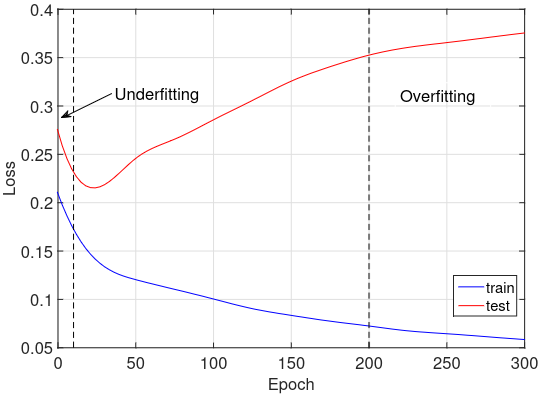
\includegraphics[width=0.4\textwidth]{img/over-under-fitting.png}
    \caption{Beispiel von Under- und Overfitting Probleme}
    \label{fig:over_under_fitting}
\end{figure}

\subsection{Overfitting}\label{sec:overfitting100}

    Overfitting tritt auf, wenn ein Modell zu stark an die Trainingsdaten angepasst ist und die Fähigkeit verliert, auf neuen, unbekannten Daten zu generalisieren. Das Modell erlernt spezifische Muster und Rauschen in den Trainingsdaten, die nicht repräsentativ für die gesamte Datenmenge sind. Dies führt zu einer übermäßigen Komplexität des Modells und einer schlechten Leistung auf neuen Daten.
    Die Ursachen für Overfitting können vielfältig sein. Eine mögliche Ursache ist eine zu große Anzahl von Parametern im Modell, die zu einer Überanpassung an die Trainingsdaten führen. Weitere Gründe können unzureichende Datenmengen, das Fehlen von Regularisierungstechniken oder das Vorhandensein von Ausreißern in den Trainingsdaten sein.
    Die Auswirkungen von Overfitting sind vielfältig und können zu suboptimalen Modellleistungen führen\footfullcite{poggio2018theory}. Das Modell kann hohe Trainingsgenauigkeit aufweisen, jedoch eine niedrige Testgenauigkeit erzielen, da es nicht in der Lage ist, das Gelernte auf neue Daten zu verallgemeinern. Dies kann zu falschen Vorhersagen und einer geringen Robustheit des Modells führen.
    Um Overfitting zu identifizieren und zu vermeiden, stehen verschiedene Techniken zur Verfügung. 
    Eine häufig verwendete Methode ist die Regularisierung, die die Komplexität des Modells reduziert und eine bessere Generalisierung ermöglicht. Beispiele für Regularisierungsmethoden sind L1- und L2-Regularisierung, die den Verlustfunktionen Strafterme hinzufügen, um große Gewichtungen zu minimieren. Dadurch wird eine bessere Kontrolle über die Modellkomplexität erreicht.
    Darüber hinaus kann das frühzeitige Beenden des Trainingsprozesses, auch bekannt als Early Stopping, dazu beitragen, Overfitting zu verhindern. Hierbei wird das Training gestoppt, wenn die Leistung auf einem Validierungsdatensatz nicht mehr verbessert wird. Dadurch wird verhindert, dass das Modell zu lange trainiert wird und sich auf spezifische Muster der Trainingsdaten spezialisiert.

\subsection{Underfitting}

    Underfitting tritt auf, wenn das Modell nicht in der Lage ist, die  Muster und Zusammenhänge in den Daten zu erfassen. 
    Es handelt sich um das Gegenteil von Overfitting, bei dem das Modell zu einfach oder zu grob ist, um die Komplexität der Daten angemessen zu modellieren. 
    Infolgedessen kann das Modell weder die Trainingsdaten noch neue Daten gut generalisieren.
    Die Gründe für Underfitting können verschiedene Ursachen haben. Eine mögliche Ursache ist die Verwendung eines zu einfachen Modells, das nicht in der Lage ist, die inhärente Komplexität der Daten abzubilden. 
    Dies kann auch auf eine unzureichende Anzahl von Parametern oder Merkmalen im Modell zurückzuführen sein. Darüber hinaus kann ein Mangel an relevanten Merkmalen oder eine unangemessene Datenpräparation zu Underfitting führen.
    Die Auswirkungen von Underfitting sind ähnlich wie bei Overfitting ungünstig. 
    Das Modell zeigt sowohl eine niedrige Trainingsgenauigkeit als auch eine niedrige Testgenauigkeit, da es nicht in der Lage ist, die Muster in den Daten adäquat zu erfassen. 
    Das Modell verliert an Informationsgehalt und seine Vorhersagen sind ungenau und wenig zuverlässig.
    Um Underfitting zu beheben, stehen verschiedene Ansätze zur Verfügung. 
    Ein erster Ansatz besteht darin, die Komplexität des Modells zu erhöhen, indem beispielsweise die Anzahl der Parameter oder die Netzwerkarchitektur erhöht wird. 
    Dies ermöglicht es dem Modell, die zugrundeliegenden Muster in den Daten besser zu erfassen.
    Dropout ist eine Technik zur Bekämpfung von Underfitting\footfullcite{liu2023dropout}. Hierbei werden zufällig einige Neuronen während des Trainings deaktiviert, um eine gewisse Redundanz im Modell zu erzeugen. Dies führt zu einer Verbesserung der Generalisierungsfähigkeit des Modells und verringert die Abhängigkeit einzelner Neuronen.
    Eine weitere Möglichkeit, Underfitting zu reduzieren, besteht darin, zusätzliche relevante Merkmale in das Modell einzubeziehen oder vorhandene Merkmale besser zu transformieren. 
    Dies kann dazu beitragen, die Modellkapazität zu erhöhen und eine bessere Passung der Daten zu ermöglichen.
    Die Anwendung von Ensemble-Methoden, bei denen mehrere Modelle kombiniert werden, kann ebenfalls dazu beitragen, Underfitting zu bekämpfen. Durch die Kombination der Vorhersagen mehrerer Modelle kann die Gesamtleistung verbessert und eine bessere Anpassung an die Daten erzielt werden.
    Es ist wichtig, die richtige Balance zwischen Overfitting und Underfitting zu finden, um ein optimales Modell zu erhalten. 
    Dies erfordert eine sorgfältige Modellauswahl und Hyperparameter-Optimierung. Eine gute Modellbewertung und Validierung auf unabhängigen Testdatensätzen sind ebenfalls entscheidend, um die Qualität des Modells zu gewährleisten.

\section{Vanishing and Exploding Gradients}

    Die Probleme der verschwindenden (vanishing) und explodierenden (exploding) Gradienten stellen eine Herausforderung beim Training von tiefen neuronalen Netzen dar. 
    Diese Phänomene können zu einer schlechten Modellleistung und einer ineffizienten Lernkonvergenz führen. 
    In diesem Kapitel werden die Ursachen dieser Probleme sowie Lösungsansätze zur Bewältigung der vanishing und exploding Gradients diskutiert.

\begin{figure}[h]
    \centering
    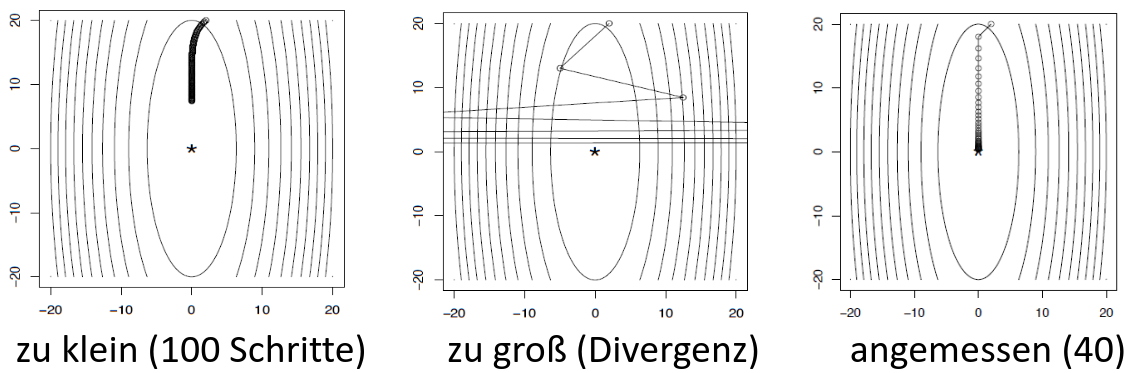
\includegraphics[width=\textwidth]{img/sgd_KI_vorlesung.png}
    \caption{Beispiel von Vanishing- und Exploding Gradient Probleme}
    \label{fig:gradient_descent_exploding_vanishing}
\end{figure}

\subsection{Ursachen der vanishing Gradients}

    Die vanishing Gradients entstehen, wenn die Gradienten während des Backpropagation-Verfahrens in tiefen neuronalen Netzen (deep neural networks) mit jedem weiteren Layer immer kleiner werden. 
    Dies tritt auf, wenn die Ableitungen der Aktivierungsfunktionen, die zur Berechnung der Gradienten verwendet werden, Werte kleiner als 1 haben.
    Die Multiplikation kleiner Zahlen in aufeinanderfolgenden Schichten führt zu exponentiell abnehmenden Gradienten.
    Ein weiterer Faktor, der vanishing Gradients verursachen kann, ist die Tiefe des neuronalen Netzes. 
    Je tiefer das Netzwerk ist, desto mehr Schichten müssen durchlaufen werden, um den Fehler zurückzupropagieren. 
    Da die Gradienten mit jeder Schicht multipliziert werden, wird ihre Größe exponentiell kleiner, was zu einem Verschwinden der Gradienten in den frühen Schichten führt.

\subsection{Ursachen der exploding Gradients}

    Im Gegensatz zu den vanishing Gradients treten bei den exploding Gradients Probleme auf, wenn die Gradienten während des Backpropagation-Verfahrens in tiefen neuronalen Netzen immer größer werden. 
    Dies geschieht, wenn die Ableitungen der Aktivierungsfunktionen Werte größer als 1 aufweisen. Die Multiplikation großer Zahlen in aufeinanderfolgenden Schichten führt zu exponentiell ansteigenden Gradienten.
    Die exploding Gradients können auch durch eine falsche Wahl der Lernrate verursacht werden. 
    Wenn die Lernrate zu hoch gewählt wird, können die Gradienten im Laufe des Trainings stark ansteigen und die Gewichte des Modells unkontrolliert verändern.

\subsection{Negative Auswirkungen der vanishing und exploding Gradients}

    Die vanishing und exploding Gradients können erhebliche negative Auswirkungen auf den Trainingsprozess und die Modellleistung haben. 
    Bei den vanishing Gradients kann die Lernkonvergenz verlangsamt werden, da die Gradienten in den frühen Schichten zu klein werden, um signifikante Gewichtsaktualisierungen zu bewirken. 
    Dadurch kann das Modell Schwierigkeiten haben, komplexe Muster und Zusammenhänge in den Daten zu erfassen.
    Bei den exploding Gradients können instabile Gewichtsaktualisierungen auftreten, die zu einer übermäßigen Anpassung des Modells an die Trainingsdaten führen können. 
    Dies kann zu einem Verlust der Generalisierungsfähigkeit des Modells führen, da es zu stark auf die Trainingsdaten spezialisiert ist.

\subsection{Lösungsansätze für vanishing Gradients}

    Um vanishing Gradients zu adressieren, stehen verschiedene Lösungsansätze zur Verfügung. 
    Eine Methode besteht darin, spezielle Initialisierungstechniken für die Gewichte zu verwenden, die eine angemessene Skalierung ermöglichen. 
    Hierbei haben sich insbesondere die Xavier-Initialisierung\footfullcite{pmlr-v9-glorot10a} und die He-Initialisierung\footfullcite{schlemper2017deep}$^{,}$\footfullcite{he2015delving} als effektiv erwiesen. 
    Diese Techniken berücksichtigen die Anzahl der Eingangs- und Ausgangsneuronen eines Layers und stellen sicher, dass die Gewichte in einem geeigneten Bereich initialisiert werden, um das Verschwinden der Gradienten zu verhindern.
    
    Eine weitere Lösung für vanishing Gradients besteht in der Verwendung geeigneter Aktivierungsfunktionen. 
    Die Rectified Linear Unit (ReLU) und die Leaky ReLU-Funktion\footfullcite{xu2017efficient} haben sich in der Praxis als wirksame Wahl erwiesen, um das Problem der verschwindenden Gradienten anzugehen. 
    Diese Aktivierungsfunktionen ermöglichen eine nicht-lineare Transformation der Eingaben und verhindern das Sättigen der Gradienten in den tiefen Schichten des Netzwerks.

\subsection{Lösungsansätze für exploding Gradients}

    Um exploding Gradients zu bewältigen, ist eine gängige Methode das Gradient Clipping\footfullcite{chen2020understanding}. 
    Dabei wird die Größe der Gradienten während des Trainings begrenzt, um zu verhindern, dass sie einen bestimmten Schwellenwert überschreiten. 
    Durch die Anwendung des Gradient Clippings wird die Stabilität des Trainingsprozesses verbessert und das Risiko von instabilen Gewichtsaktualisierungen reduziert.
    Eine weitere Möglichkeit, exploding Gradients zu vermeiden, besteht darin, die Lernrate anzupassen\footfullcite{qiao2015fast}. 
    Es kann hilfreich sein, adaptive Optimierungsalgorithmen wie den Adam-Optimizer zu verwenden, der automatisch die Lernrate für jedes Gewicht anpasst. 
    Durch die dynamische Anpassung der Lernrate werden große Gewichtsaktualisierungen vermieden und die Konvergenz des Modells verbessert.

\section{Gradient Descent Optimization}

    Der Abschnitt "Gradient Descent Optimization" behandelt die Herausforderungen und Lösungen im Bereich der Optimierungsalgorithmen\footfullcite{ruder2016overview} für das Gradientenabstiegsverfahren, die in der Praxis bei der Schulung tiefer neuronaler Netze häufig eingesetzt werden. 
    Dieser Abschnitt bietet einen Überblick über die gängigsten Optimierungsalgorithmen und deren Auswirkungen auf die Effizienz und Konvergenzgeschwindigkeit des Trainingsprozesses.

\subsection{Standard-Gradientenabstieg}

    Der Standard-Gradientenabstieg\footfullcite{wanto2018analysis} ist der grundlegende Optimierungsalgorithmus, der zur Aktualisierung der Gewichte in neuronalen Netzen verwendet wird. 
    Bei diesem Verfahren wird der Gradient der Verlustfunktion für jeden einzelnen Trainingsdatensatz berechnet und die Gewichte entsprechend angepasst. 
    Obwohl der Standard-Gradientenabstieg einfach zu implementieren ist, hat er einige Herausforderungen.
    Ein Problem des Standard-Gradientenabstiegs ist seine langsame Konvergenzgeschwindigkeit. 
    Da der Gradient für jeden Trainingsdatensatz separat berechnet wird, kann dies zu einer ineffizienten Aktualisierung der Gewichte führen. 
    Darüber hinaus besteht die Gefahr von lokalen Minima oder Plateaus, in denen das Modell stecken bleiben kann und Schwierigkeiten hat, sich weiter zu verbessern.

\subsection{Stochastischer Gradientenabstieg (SGD)}

    Eine verbreitete Verbesserung des Standard-Gradientenabstiegs ist der stochastische Gradientenabstieg (SGD). 
    Beim SGD wird der Gradient nicht für jeden einzelnen Trainingsdatensatz berechnet, sondern nur für eine zufällig ausgewählte Teilmenge der Daten, auch als Mini-Batch bezeichnet\footfullcite{khirirat2017mini}. 
    Dadurch wird der Trainingsprozess beschleunigt, da weniger Berechnungen erforderlich sind.
    Der SGD bietet jedoch auch Herausforderungen. 
    Er kann zu einer instabilen Aktualisierung der Gewichte führen, da die zufällige Auswahl der Mini-Batches zu einer großen Varianz in den Gradientenschätzungen führen kann. 
    Dies kann zu einer schlechten Konvergenz und einer inkonsistenten Modellleistung führen.

\subsection{Mini-Batch Gradientenabstieg}

    Um die Vorteile des SGD zu nutzen und gleichzeitig die Stabilität zu verbessern, wird oft der Mini-Batch Gradientenabstieg eingesetzt\footfullcite{khirirat2017mini}.
    Beim Mini-Batch Gradientenabstieg werden die Gradienten auf der Grundlage einer Mini-Batch-Größe berechnet, die größer als eins ist, aber kleiner als die gesamte Trainingsdatenmenge. 
    Dadurch werden sowohl die Effizienz als auch die Stabilität des Trainingsprozesses verbessert.

\subsection{Batch Normalisierung}

    Ein weiterer Ansatz zur Verbesserung des Gradientenabstiegs besteht in der Batch-Normalisierung\footfullcite{cai2019quantitative}. 
    Dieses Verfahren normalisiert die Eingabeaktivierungen eines Netzwerks innerhalb eines Mini-Batches, um die interne Covariate Shift-Problematik zu reduzieren. 
    Die Batch-Normalisierung verbessert die Konvergenz des Modells, indem sie die Gradientenflüsse stabilisiert und die Abhängigkeit von der Initialisierung der Gewichte verringert.
